% =====================================================================
% VERSION ENSAE, REDUCTION SFE (phase 3, 1er octobre 2026) : chapitre 9, resultats.
% Copie a texte constant de chapitres/12_resultats.tex.
% Ne changent que les titres et les renvois repares, listes dans
% reduction/phase3.md.
% Lu par main_ensae.tex seul : ne jamais le faire lire par main_institut.tex,
% qui garde chapitres/.
% =====================================================================

\chapter{Résultats}
\label{chap:resultats}
\label{part:resultats}

Pour chaque état de conformité, le moteur fixe quatre paramètres : la fréquence $\lambda$, la probabilité de dépassement
$p_u$, le gain de propagation $g$ et la probabilité de choc commun $\omega$
(chapitre~\ref{chap:multietats}). Il tire les incidents, les piliers atteints et leurs pertes,
puis calcule le quantile à $99{,}5\,\%$ de la somme annuelle. Les comparaisons utilisent le même
moteur, les mêmes graines et la même loi de sévérité de base dans le scénario principal ; les
calculs d'entité emploient le protocole distinct du \S\ref{sec:ancrage}.

Trois lectures doivent accompagner le résultat : l'écart entre états quand les quatre canaux
changent ensemble (\S\ref{sec:chiffre-de-tete}), son déplacement quand on change le coût d'un
incident (\S\ref{sec:institut-unite-perte}) et son incertitude de calibration
(\S\ref{sec:institut-bootstrap-joint}). Les attributions et les cas d'usage se lisent sous ces
conditions. Les montants concernent le périmètre financier étudié : leur niveau varie d'un
facteur $41$ selon sévérité et fréquence, contre au plus $33\,\%$ de leur moyenne pour les
rapports au socle (chapitre~\ref{chap:partielle}). Nous comparons OpRisk ($\hat\xi=0{,}595$)
et PRC ($\hat\xi=1{,}03$), plafonnée à $40$~M\euro{} par perte élémentaire.
% SOURCES-SCRIPTS: 65 66 12 16 63

\section{Besoin de capital par état de conformité}

\subsection*{Scénario principal et remédiations partielles}
\label{sec:chiffre-de-tete}

La comparaison principale modifie les quatre canaux. Les autres lignes reprennent des protocoles
partiels : le score seul garde $g$ au niveau NC ; les combinaisons à deux et trois canaux
correspondent aux lectures B et C du tableau~\ref{tab:scretat}.
Ces niveaux ne sont pas les configurations intermédiaires du calcul à quatre canaux.
À trois canaux, l'état conforme vaut $5\,932$~M\euro{} ; à quatre
canaux, $6\,049$~M\euro{}. Ces deux états conservent une contagion, ce qui les distingue du
socle $5\,275$~M\euro{} calculé sans contagion au chapitre~\ref{chap:partielle}.

\begin{center}\footnotesize
\renewcommand{\arraystretch}{1.25}
\begin{tabular}{@{}l c r r r@{}}
\toprule
\textbf{Lecture} (besoin à $99{,}5\,\%$, M\euro, états posés) & \textbf{canaux} & \textbf{conforme} & \textbf{non conf.} & \textbf{facteur} \\
\midrule
Score de conformité seul, $g$ figé au niveau NC & 1 & 7987 & 16\,847 & $2{,}11$ \\
Fréquence $+$ propagation (lecture~B) & 2 & 6664 & 15\,074 & $2{,}26$ \\
$+$ détection (lecture~C) & 3 & 5932 & 16\,595 & $2{,}80$ \\
\textbf{$+$ accumulation P4 (les quatre canaux)} & \textbf{4} & \textbf{6049} & \textbf{20\,188}
& $\mathbf{3{,}34}$ \\
\bottomrule
\end{tabular}
\end{center}

\vspace{4pt}
\noindent Pour le périmètre financier étudié, la lecture à quatre canaux donne
$6\,049\to20\,188$~M\euro, soit un facteur $3{,}34$ et un écart de $14\,139$~M\euro{} : écart-type
$734$~M\euro{} entre quatre graines, erreur type de la moyenne $367$~M\euro.
Le score seul diffère de la lecture à fréquence variable (A) du tableau~\ref{tab:scretat}.
Les lectures B et C excluent le choc commun P4. La détection ajoute $2\,928\pm343$~M\euro{}
en Shapley, $4\,562\pm819$ en fermeture (figure~\ref{fig:canaux-rapport}), signe constant sur seize graines.
Le facteur compare deux états posés, sans mesurer un effet causal de DORA. Toute remédiation
partielle s'évalue depuis l'état de départ, avec ses interactions.

% SOURCES-SCRIPTS: 25 16 43 67 68 74 30


\subsection*{Détail des lectures partielles}

Le tableau~\ref{tab:scretat} distingue la fréquence variable seule (A), l'ajout de la propagation
(B), puis de la détection (C). Le besoin augmente de l'état conforme à l'état non conforme
dans chaque lecture. Les lettres renvoient uniquement à ces combinaisons de canaux.

\begin{table}[htbp]\centering\small
\renewcommand{\arraystretch}{1.25}
\begin{tabular}{@{}l ccc c ccc@{}}
\toprule
& \multicolumn{3}{c}{\textbf{OpRisk} (M\euro)} & & \multicolumn{3}{c}{\textbf{PRC} (M\euro)} \\
\cmidrule(lr){2-4}\cmidrule(lr){6-8}
État & Fréq. & $+$ prop. & $+$ dét. & & Fréq. & $+$ prop. & $+$ dét. \\
\midrule
Conforme               & 8301  & 6664  & 5932  & & 2589 & 1903 & 1642 \\
Partiellement conforme & 11059 & 9625  & 9625  & & 3653 & 3118 & 3118 \\
Non conforme           & 15074 & 15074 & 16595 & & 5520 & 5520 & 6577 \\
\bottomrule
\end{tabular}
\caption{Besoin de capital par état, trois lectures (A~: fréquence ; B~: $+$~propagation ; C~:
$+$~détection), sans le canal d'accumulation. Le canal détection ne joue qu'aux extrêmes (il
% SOURCES-SCRIPTS: 16
abaisse l'état conforme et relève le non conforme), l'état partiel n'étant pas modulé.}
\label{tab:scretat}
\end{table}

\begin{figure}[H]\centering
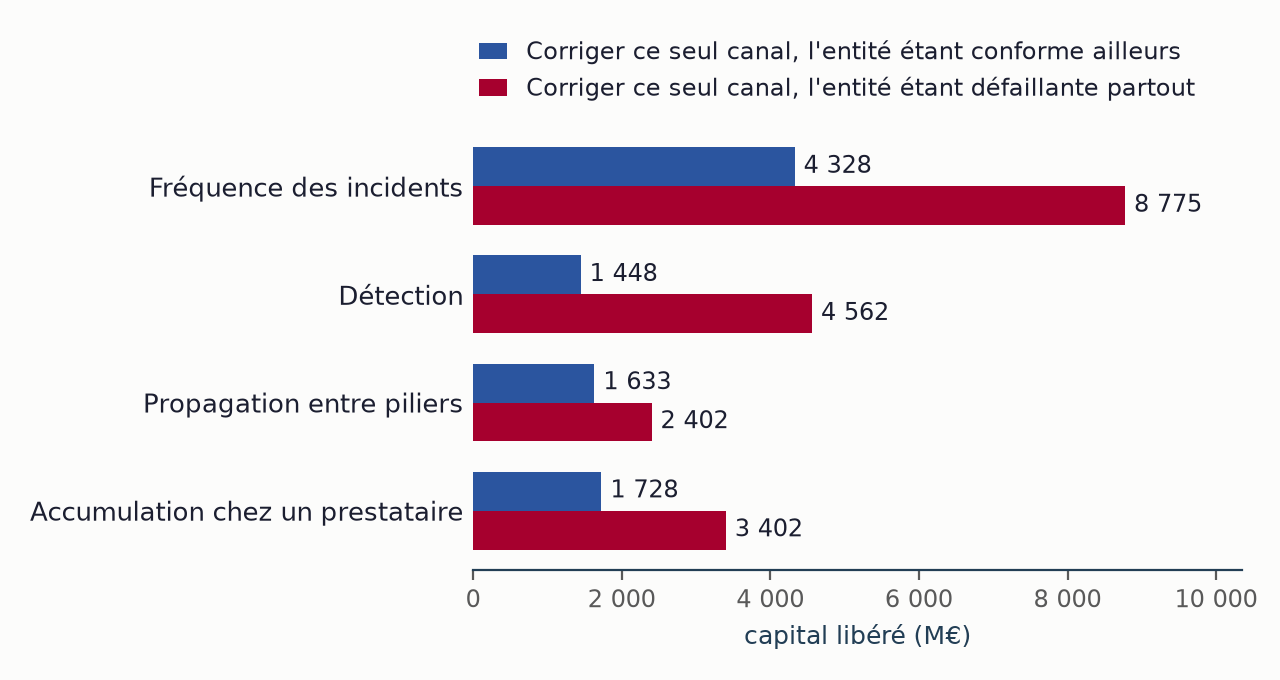
\includegraphics[width=0.72\textwidth]{N1_canaux_note.png}
\caption{Capital libéré par la correction d'un seul canal, selon que l'entité est déjà conforme sur
les trois autres canaux (effet isolé) ou défaillante partout (effet de fermeture), en M\euro{} à
l'échelle du secteur.}
% SOURCES-SCRIPTS: 101 68
\label{fig:canaux-rapport}
\end{figure}

Les protocoles reposent sur des bases différentes. Du score seul à la combinaison fréquence et
propagation, l'écart passe de $8\,860$ à $8\,410$~M\euro{} alors que le facteur monte, la
base conforme passant de $7\,987$ à $6\,664$~M\euro. Les canaux se multiplient presque, le produit
des quatre facteurs isolés étant de $3{,}47$ pour un facteur publié de $3{,}34$
(figure~\ref{fig:treillis-canaux-rapport}). Les quatre effets isolés somment à $9\,138$~M\euro{} et
l'écart de $14\,139$ les dépasse de $5\,001$, l'interaction. Elle correspond à ce que donnerait un
produit des facteurs ($5\,813$~M\euro{} pour un modèle purement multiplicatif) plus qu'à un effet
propre de la cascade (\S\ref{sec:inverse}). Les
trajectoires et la priorisation restent conduites en lecture~B, car elles concernent l'ordre de
remédiation, que le canal ajouté ne déplace pas.

\begin{figure}[H]\centering
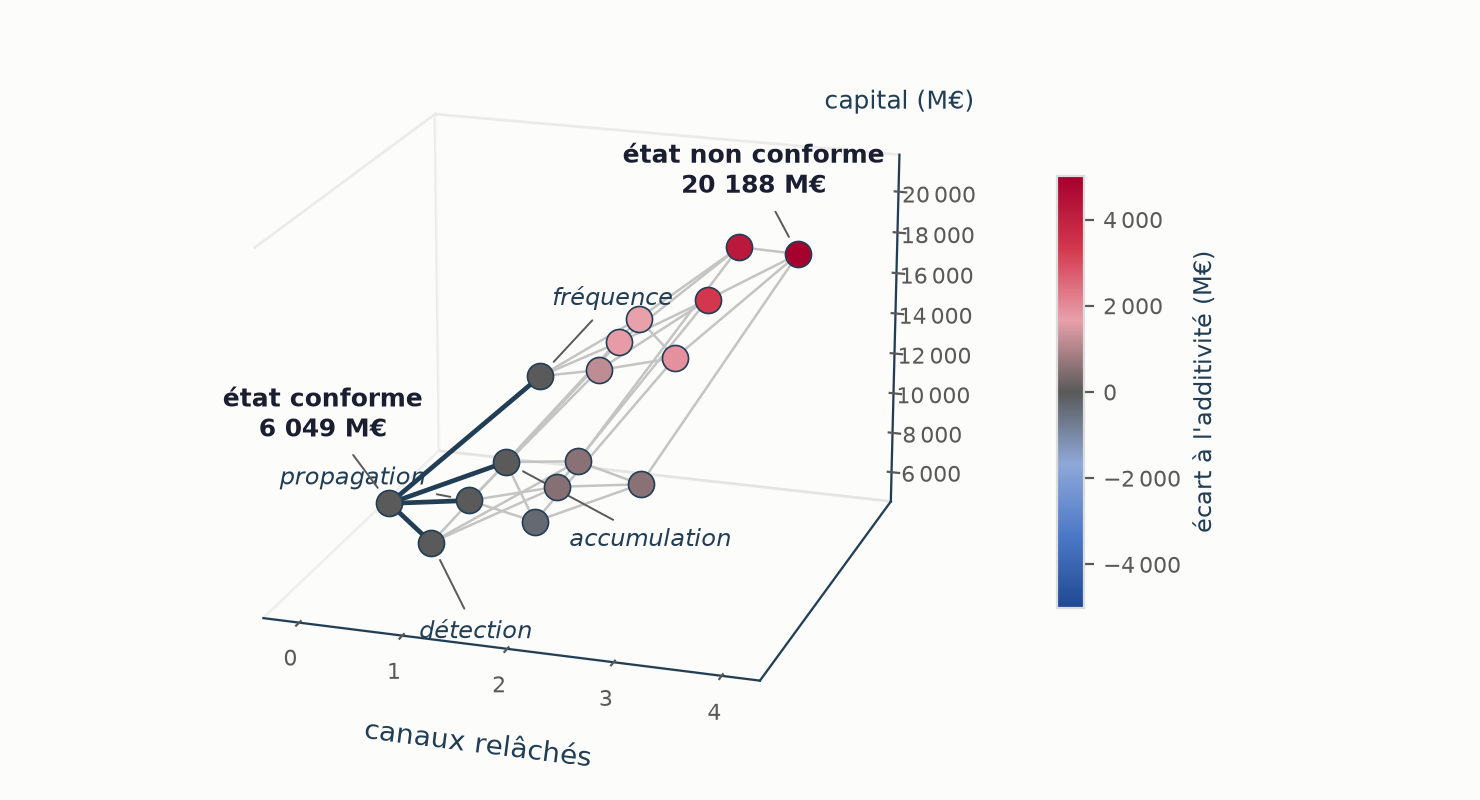
\includegraphics[width=0.95\textwidth]{treillis_canaux.png}
\caption{Les seize configurations des quatre canaux, rangées par nombre de canaux relâchés. La
hauteur est le capital ; les deux extrémités sont les états publiés, $6\,049$ et
$20\,188$~M\euro{}, et tout sommet intermédiaire est une remédiation partielle. Chaque arête monte.
La couleur est l'écart à l'additivité, capital observé moins la somme des quatre effets isolés :
$+5\,001$~M\euro{} au sommet complet, $-330$ sur la seule paire négative, propagation et
accumulation. Le troisième axe sépare les configurations de même rang et ne porte aucune grandeur.}
% SOURCES-SCRIPTS: 68 108
\label{fig:treillis-canaux-rapport}
\end{figure}

Nous obtenons le surcoût $\Delta_{\text{DORA}}=B(\text{NC})-B(\text{C})$, à
graine Monte-Carlo commune, par bootstrap à deux niveaux (multiplicateurs et sévérité), et
$100\,\%$ des tirages sont positifs (tableau~\ref{tab:delta}).

\begin{table}[htbp]\centering\small
\renewcommand{\arraystretch}{1.25}
\begin{tabular}{@{}l cc@{}}
\toprule
& médiane & IC90\,\% \\
\midrule
$\Delta_{\text{DORA}}$ NC vs C (OpRisk) & 6476 & $[2940\,;47368]$ \\
$\Delta_{\text{DORA}}$ PC vs C (OpRisk) & 2346 & $[1137\,;13566]$  \\
$\Delta_{\text{DORA}}$ NC vs C (PRC)    & 3668 & $[3201\,;4094]$  \\
$\Delta_{\text{DORA}}$ PC vs C (PRC)    & 1257 & $[1077\,;1466]$  \\
\bottomrule
\end{tabular}
\caption{Surcoût de non-conformité (M\euro), lecture B, bootstrap deux niveaux. Côté OpRisk la
sévérité de queue est ré-échantillonnée sur les $86$ excès réels ; l'intervalle reste large parce
que la queue l'est.}
\label{tab:delta}
\end{table}

L'intervalle large côté OpRisk est la signature d'une queue d'indice $0{,}60$, et le surcoût est positif dans tous les tirages. Il porte sur la lecture B. L'écart à quatre canaux est accompagné ici de sa dispersion entre graines (écart-type de $734$~M\euro) ; le bootstrap conjoint de la section~\ref{sec:institut-bootstrap-joint} traite son incertitude de calibration. Lorsqu'on
réinjecte le résidu de la conversion de \citet{jacobs2014}, $0{,}523$ en logarithme, c'est-à-dire un
facteur $2{,}4$ à $90\,\%$ autour de la droite, l'intervalle PRC reste étroit et le niveau du
surcoût bouge de $7\,\%$.

% SOURCES-SCRIPTS: 25 16 43 67 68 100 14 21 74

\section{Décomposition et allocation par pilier}
\label{sec:allocation}

Si l'on bascule un pilier à la fois de conforme à non conforme, le surcoût se décompose selon le
classement $P1>P4>P2>P3>P5$, celui du classement ROOT du modèle qualitatif. Cet accord est attendu et
ne constitue pas une validation indépendante, car les amorces de la cascade sont semées selon ROOT, posé par le même expert que
la matrice dont $W$ est tirée (\S\ref{sec:baremes}).

Les surcoûts isolés ne somment pas au surcoût total, la différence étant une interaction qu'un modèle sans
propagation ne produit pas. Sur la VaR à $99{,}5\,\%$ OpRisk, son signe n'est pas résolu, de $-137$ à
$+1\,395$~M\euro{} sur six graines de $60\,000$ années, positive quatre fois sur six. Elle est
positive sur les six graines en perte moyenne, de $+532$ à $+659$~M\euro{} côté OpRisk et $+827$
côté PRC, et dans la VaR du périmètre PRC, dont le plafond tronque la queue ($+905$~M\euro).

L'attribution par pilier exige donc une règle additive, la valeur de Shapley. Cette
interaction entre piliers ne s'additionne pas à l'interaction de $+5\,001$~M\euro{} entre les quatre
canaux, de signe résolu (\S\ref{sec:kpi}). Elles décomposent l'écart selon deux axes, les piliers et
les canaux, et l'attribution par pilier se lit sur le protocole du tableau~\ref{tab:shapley}.
% SOURCES-SCRIPTS: 16b 20b 68

Shapley répartit l'écart de capital entre les piliers
dont la non-conformité est modifiée, en incluant les interactions. Euler, dans le calcul retenu ici,
répartit la perte moyenne au-delà du quantile entre les piliers touchés ; ses contributions somment
à cette moyenne de pertes extrêmes. Ces deux lectures portent sur des objets distincts et
ne fournissent pas le même budget de remédiation.
% SOURCES-SCRIPTS: 20

\subsection{Attribution par Shapley}

On munit les piliers d'une fonction caractéristique
\[
v(S) \;=\; B\bigl(S \text{ en NC},\ \text{reste C}\bigr)-B(\text{tous C}),
\qquad S \subseteq \{P1,\dots,P5\},
\]
calculée par la cascade sur les $2^5$ configurations à graine Monte-Carlo commune. La valeur de
Shapley
\[
\varphi_j \;=\; \sum_{S \subseteq \{P1,\dots,P5\}\setminus\{j\}}
\frac{|S|!\,\bigl(5-|S|-1\bigr)!}{5!}\,\bigl[v(S\cup\{j\})-v(S)\bigr]
\]
moyenne la contribution de $j$ sur tous les ordres d'arrivée. Ici $S$ est une coalition de piliers et $|S|$ son effectif ; ce $S$ diffère de la partie symétrique de $W$. Ainsi
$\sum_j \varphi_j = v(\text{tous}) = \Delta_{\text{DORA}}$ \citep{Shapley1953}. Son
emploi en allocation de capital remonte à \citet{denault2001}, et son usage actuariel sous
Solvabilité~II est documenté \citep{Decupere2011}. Avec cinq piliers, on énumère les $5!$
ordres, sans les algorithmes par échantillonnage \citep{CastroGomezTejada2009, SongNelsonStaum2016}.
Le tableau~\ref{tab:shapley} en donne les valeurs.

\begin{table}[H]\centering\small
\renewcommand{\arraystretch}{1.25}
\begin{tabular}{@{}l rrr c rrr@{}}
\toprule
& \multicolumn{3}{c}{OpRisk} & & \multicolumn{3}{c}{PRC} \\
\cmidrule{2-4}\cmidrule{6-8}
pilier & marginal & $\varphi_j$ & part & & marginal & $\varphi_j$ & part \\
\midrule
P1 gouvernance & 3481 & 3717 & $34{,}0\,\%$ & & 1375 & 1608 & $32{,}4\,\%$ \\
P4 tiers       & 2658 & 2810 & $25{,}7\,\%$ & & 1075 & 1252 & $25{,}3\,\%$ \\
P2 incidents   & 1634 & 1867 & $17{,}1\,\%$ & &  721 &  920 & $18{,}6\,\%$ \\
P3 tests       & 1094 & 1484 & $13{,}6\,\%$ & &  571 &  738 & $14{,}9\,\%$ \\
P5 partage     &  665 & 1048 &  $9{,}6\,\%$ & &  311 &  438 &  $8{,}8\,\%$ \\
\midrule
somme          & 9531 & 10\,927 & $100{,}0\,\%$ & & 4052 & 4957 & $100{,}0\,\%$ \\
\bottomrule
\end{tabular}
\caption{Valeur de Shapley du surcoût $\Delta_{\text{DORA}}$ (M\euro, périmètre financier étudié, trois canaux : fréquence, propagation, détection ; base
conforme $6\,085$ du moteur par pilier, qui s'écarte de quelques pour cent de la lecture~C du tableau~\ref{tab:scretat}).}
% SOURCES-SCRIPTS: 16b
\label{tab:shapley}
\end{table}

Le classement de Shapley reproduit le classement ROOT sur les deux périmètres, en partie
mécaniquement, les amorces étant semées selon ROOT (parts $30/27/18/15/9\,\%$). La part de P1,
$34\,\%$, excède toutefois sa part d'amorce de $30\,\%$, ce qui traduit l'effet propre de la
propagation, P1 étant l'émetteur le plus fort de $W$.
% SOURCES-SCRIPTS: 20

\subsection{Allocation par Euler}

La règle d'Euler \citep{tasche1999} calcule
$C_j = \mathbb{E}\bigl[L_j \mid L \ge \VaR_{99{,}5\,\%}\bigr]$, où $L_j$ est la perte annuelle attribuée au pilier $j$, avec $L=\sum_j L_j$. Ces contributions somment à $\TVaR_{99{,}5\,\%}(L)$ et non au quantile : c'est une allocation de
la moyenne de queue, lue comme diagnostic de la localisation du capital. Côté PRC, l'allocation est stable et presque plate (P2 $23\,\%$, P4 $23\,\%$, P1 $20\,\%$, P3
$18\,\%$, P5 $17\,\%$), le plafond de sévérité tronquant la queue ($\TVaR = 6\,795 \approx \VaR =
6\,573$~M\euro). Côté OpRisk, les parts moyennes sont stables, mais l'allocation de la queue
extrême ne l'est pas. En effet, avec $\xi \approx 0{,}6 > 0{,}5$, la sévérité est de variance infinie
et le classement conditionnel bascule d'une résolution de simulation à l'autre. Nous retenons donc
l'allocation du périmètre PRC.
% SOURCES-SCRIPTS: 16b

Le besoin de capital publié est partout le quantile $\VaR_{99{,}5\,\%}(L)$ non centré, la perte
attendue d'une non-conformité n'étant pas couverte par une provision. Aucune grandeur de couverture
n'est une TVaR. La mesure de queue ne sert qu'au diagnostic, à deux titres. Elle sert d'abord de
base à l'allocation d'Euler, qui répartit la TVaR et non le quantile. Elle indique aussi la forme de la queue, le rapport
$\TVaR_{99{,}5\,\%}(L)/\VaR_{99{,}5\,\%}(L) \approx 2{,}1$ se comparant à son asymptote
$1/(1-\xi) = 2{,}5$. Ce rapport est de $2{,}10$ à l'état tous non conforme et de $2{,}17$ sur la
calibration de référence. Sous la calibration PRC non plafonnée, $\hat\xi=1{,}033>1$ rend l'espérance infinie :
la mesure de queue n'existe pas et ne peut fonder un besoin de capital. L'allocation du
périmètre PRC porte sur la sévérité plafonnée, dont les moments sont finis.
% SOURCES-SCRIPTS: 20 67 73

\section{Trajectoire du capital et ordre de remédiation}
\label{sec:res-traj}

Le long de la mise en conformité, en lecture~B, le capital OpRisk passe de $10\,752$ à $7\,041$~M\euro{}
en cinq ans, vers le besoin de l'état conforme. La trajectoire part d'une répartition supposée des
états (NC~$35\,\%$, PC~$35\,\%$, C~$30\,\%$). Le surcoût résiduel tend vers zéro, et son intégrale, à un coût de capital près, est le
coût de portage de la non-conformité pendant la remédiation. La bande à $90\,\%$ reste haute en
environnement dégradé, scénario où le capital importe le plus.
% SOURCES-SCRIPTS: 17

\label{sec:res-prio}%
Sous budget contraint, un pilier remédié à la fois, nous énumérons les $120$ ordres, dont
l'optimal, $P1\to P4\to P2\to P3\to P5$, est égal à l'ordre ROOT et distinct de l'ordre glouton par
valeur d'accélération. L'écart de capital intégré entre le pire ordre et l'optimal atteint
$21\,\%$. Remédier au coup par coup le pilier au plus fort gain immédiat coûte plus cher, car les
interactions de cascade imposent de raisonner sur l'horizon entier.
% SOURCES-SCRIPTS: 18

Le test de résistance inverse fixe le capital et cherche les états qui le produisent, la monotonie
du \S\ref{sec:kpi} rendant croissant l'ensemble des configurations atteignant une cible, donc décrit
par ses éléments minimaux. Le canal de fréquence seul atteint $10\,377$~M\euro, soit $1{,}72$ fois
l'état conforme, et les trois autres canaux réunis n'atteignent que $11\,413$ ($1{,}89$ fois).
Toute cible sous le premier seuil se produit par un canal unique, et toute cible au-dessus du second
exige la fréquence. Aucun autre canal seul n'atteint $8\,000$~M\euro{} (\S\ref{sec:inverse}).
% SOURCES-SCRIPTS: 92

\section{Comparaison aux copules et à la Formule Standard}
\label{sec:benchmark}

Comme la cascade remplace l'agrégation par copule d'un modèle LDA, nous la confrontons à des modèles à copule
de mêmes marges par pilier, à graines communes, sur le périmètre OpRisk. À corrélation
calée, la copule gaussienne retombe sur le besoin de capital de la cascade ($+0{,}1\,\%$ sur une graine,
$+4{,}8\,\%$ en moyenne sur quatre, sous son propre bruit). En queue lourde, le quantile annuel
tient à la perte unique dominante, et le niveau n'identifie pas la dépendance. La Student
($\nu = 4$) le surestime de $17\,\%$ en forçant des co-extrêmes que la cascade ne produit pas
($2{,}28$ piliers extrêmes par année de queue contre $1{,}12$). Le préprint de cascade climatique
\citep{ccrn2026} emploie le même protocole.

Basculer un pilier en non-conformité est cependant une intervention. Le comparateur construit ici
garde la même matrice de corrélation dans tous les états ; il donne un surcoût inférieur de
$38\,\%$, $6\,760$~M\euro{} contre $10\,927$ pour la cascade, faute de mécanisme de propagation dans
cette spécification. Une copule dont la dépendance varierait avec l'état n'a pas été testée. Son interaction moyenne est nulle par construction, tandis que la
cascade en produit $+560$~M\euro{}. La priorité qu'il implique s'inverse sur P2 et P3. Sa dépendance
ne durcit pas non plus lorsque la conformité se dégrade, alors que c'est le canal de propagation que la non-conformité
déplace ($g$ de $0{,}45$ à $0{,}90$).
% SOURCES-SCRIPTS: 23 80 67

\label{sec:regard-reglementaire}%
Sur le même écart de capital entre profil conforme et profil non conforme, trois cadres expriment des
fractions différentes de l'effet de la conformité (tableau~\ref{tab:benchmark-sf}).

\begin{table}[H]\centering\small
\renewcommand{\arraystretch}{1.25}
\begin{tabular}{@{}l r r@{}}
\toprule
\textbf{Cadre} & \textbf{$\Delta$ capital C$\to$NC} & \textbf{part de l'effet cascade} \\
\midrule
Formule Standard (Solvabilité~II) & $0$~M\euro{} & $0\,\%$ \\
LDA-copule gaussienne figée (comparateur) & $6\,760$~M\euro{} & $62\,\%$ \\
Cascade dirigée & $10\,927$~M\euro{} & $100\,\%$ (référence) \\
\bottomrule
\end{tabular}
\caption{Fraction de l'effet DORA que chaque cadre sait exprimer (périmètre financier étudié, trois
canaux, accumulation exclue, protocole du tableau~\ref{tab:shapley}).}
\label{tab:benchmark-sf}
\end{table}

La charge de risque opérationnel de l'équation~\eqref{reg:eq:scrop} ne dépend que du volume. Elle
est identique pour une entité exemplaire et pour une entité défaillante sur DORA. Le comparateur à
copule figée restitue $62\,\%$ de l'écart simulé, par les canaux fréquence et détection, mais pas
la propagation. Ce rapport caractérise cette spécification, non l'ensemble des modèles à copule.
% SOURCES-SCRIPTS: 27 67

\section{Méthode de descente à l'échelle d'une entité}
\label{sec:ancrage}

La descente d'échelle (\emph{downscaling}) adapte le nombre d'incidents et le montant des pertes aux actifs de l'entité, puis recalcule la distribution annuelle et son quantile. Les actifs mesurent ici la taille ;
les fonds propres mesurent la capacité d'absorption. Le métier n'a pas de coefficient estimé.
Pour l'entité notionnelle, le repère forfaitaire de la Formule Standard est d'environ $450$~M\euro. Le socle sans contagion du périmètre financier étudié vaut $5\,275$~M\euro{} ;
les deux ne se comparent pas.
% SOURCES-SCRIPTS: 60 49

\subsection{Calibration de référence sur les actifs}

Au niveau du
sinistre unique, le quantile de sévérité ($663$~M\euro) et sa moyenne de queue ($1\,752$~M\euro)
sont en revanche du même ordre que les grandes pertes cyber observées ($1\,288$ à $2\,208$~M\euro). Les calculs d'entité changent de protocole : ils emploient la
cascade indépendante de l'évaluateur du chapitre~\ref{chap:partielle}, sans choc commun P4, et
seul le gain de propagation y varie entre états. À matrice $W$ inchangée, une entité d'actifs $A$
reçoit une fréquence et une sévérité lues à sa taille :
\begin{equation}\label{eq:descente}
\begin{gathered}
\lambda(A)=\lambda_0\Big(\frac{A}{A_0}\Big)^{b_\lambda},\qquad
m(A)=\Big(\frac{A}{A_m}\Big)^{b},\\
X=m(A)\sum_{k\in S_a}Y_k,\qquad
B(A)=\VaR_{99{,}5\,\%}\Big(\sum_{n=1}^{N}X_n\Big),
\end{gathered}
\end{equation}
où le panel est formé des firmes du secteur financier dont les actifs sont connus, sur
$2005$--$2022$, et de leurs pertes des sous-catégories liées aux systèmes d'information et aux prestataires.
La fréquence y est ajustée par une binomiale négative à lien logarithmique sur les seules firmes de plus de
$100$~Md\$ d'actifs ($6\,048$ lignes, $1\,402$ firmes) : $b_\lambda=0{,}494$ (erreur-type $0{,}066$ par grappes de firmes),
$A_0=570$~Md\$ est la moyenne géométrique de leurs actifs et $\lambda_0$ la fréquence à cette taille.

$N$ suit cette binomiale négative de moyenne $\lambda(A)$, $S_a$ est
l'ensemble des piliers touchés depuis l'amorce $a$, et les $Y_k$ sont les sévérités élémentaires : la GPD
calibrée au-delà du seuil, un tirage parmi les $484$ pertes observées sous le seuil sinon. $A_m$ est la taille
médiane des pertes retenues, $b=0{,}087$ l'élasticité de la sévérité, d'où $m = 0{,}854$ à la taille de l'entité
notionnelle. Cette élasticité est estimée sur les pertes TIC du panel, corrigée de la troncature
(\S\ref{sec:biais-chiffres}) ; l'appliquer à la sévérité cyber-finance du modèle est une hypothèse de
transfert, qui s'ajoute à son incertitude d'estimation.

Sur tout le panel, $b_\lambda$ vaut $0{,}074$ : la fréquence dépendrait à peine des actifs. Une firme y
est observée de la première à la dernière année où elle apparaît dans la base, pour un risque quelconque.
Les firmes de moins de $1$~Md\$ d'actifs le sont $1{,}44$ an en moyenne, celles de plus de $100$~Md\$
$4{,}31$ ans, ce qui rend plausible un biais de fenêtre. Il n'est pas démontré : $57{,}8\,\%$ des grandes
firmes ne sont observées qu'un an, et une année sans événement enregistré n'est pas une année sans incident.
L'exposant monte avec le seuil de taille : $0{,}139$ au-delà de $1$~Md\$, $0{,}269$ au-delà de $10$~Md\$,
$0{,}494$ au-delà de $100$~Md\$ et $0{,}513$ au-delà de $300$~Md\$. À fenêtre d'au moins cinq ans, il vaut
$0{,}223$ sur tout le panel et $0{,}530$ sur les grandes firmes ; un effet fixe d'année ne le déplace pas
($0{,}497$). Nous retenons la valeur à $100$~Md\$ comme variante privilégiée sous ces hypothèses ; elle est
extrapolée aux entités plus petites, et c'est la réserve principale de cette lecture. La sévérité ne croît pas avec la
taille : sur les $521$ pertes dont les actifs sont connus, la pente de la perte sur la taille est de $-0{,}07$
(erreur-type $0{,}03$), et elle reste négative parmi les firmes de plus de $50$~Md\$.

Cette lecture remplace, après le dépôt du rapport ENSAE, la lecture du registre et les deux conventions
d'exposition de la version précédente. Elle lève le gel de la calibration pour la seule partie entité ;
les résultats du périmètre financier ne changent pas. Avec l'exposant et le moteur de la version
précédente, le même script redonne les $169{,}0$~M\euro{} publiés.

\begin{table}[htbp]\centering
\small
\begin{tabular}{lrrrr}
\toprule
Lecture & $\lambda$ (an$^{-1}$) & sévérité & Besoin à $99{,}5\,\%$ & Perte moyenne \\
\midrule
Périmètre financier étudié & $21{,}56$ & $\times 1$ & $8\,123$~M\euro & $983$~M\euro \\
Seuil \og{}$\geq 10$ événements\fg{} & $0{,}210$ & $\times 1$ & $488$~M\euro & $9{,}7$~M\euro \\
Seuil \og{}toutes firmes\fg{} & $0{,}100$ & $\times 1$ & $229$~M\euro & $4{,}6$~M\euro \\
Registre, $\lambda$ lu à la taille de la cible & $0{,}092$ & $\times 1$ & $198$~M\euro & $4{,}3$~M\euro \\
Registre, deux canaux composés & $0{,}092$ & $\times 0{,}854$ & $169$~M\euro & $3{,}6$~M\euro \\
\textbf{Lecture retenue} & $\mathbf{0{,}021}$ & $\mathbf{\times 0{,}854}$ &
$\mathbf{24}$~M\euro & $\mathbf{0{,}85}$~M\euro \\
\bottomrule
\end{tabular}
\caption{Comparaison des lectures d'échelle. Les lignes historiques adaptent la fréquence et l'échelle
de sévérité ; celles du registre emploient l'exposant $0{,}074$. La dernière réestime la fonction de
fréquence et la dispersion sur les grandes institutions et inclut les pertes observées sous le seuil.
Les lignes sont des lectures d'échelle, non des entités observées.}
\label{tab:echelle}
\end{table}

Diviser $\lambda$ par $1\,031$ divise la perte moyenne par $1\,158$ et le capital par $336$. Le chiffre
d'entité est une bande, $[15{,}8\,;27{,}5]$~M\euro{} sur les $1\,024$ sommets admissibles, qui ne traduit
que l'ignorance de la direction. Un bootstrap par firme réestimant intercept, pente et dispersion
donne $[8{,}3\,;53{,}0]$~M\euro{}, à sévérité et graine fixées ; la pente seule, à $\pm 1{,}96$ fois
l'ancienne erreur-type hessienne de $0{,}043$, donne $[12{,}3\,;41{,}9]$. Aucune de ces bandes ne corrige
la sélection du registre. Estimée au-delà de $300$~Md\$, la fréquence donne $20{,}6$~M\euro. Les
$24$~M\euro{} restent une extrapolation d'ordre de grandeur (\S\ref{sec:entites-reelles}).

La baisse depuis $169$~M\euro{} ne tient pas à l'exposant seul. Sur les huit combinaisons de fréquence,
de dispersion et de pertes sous le seuil, à nombres communs et sur quatre graines, la nouvelle fréquence
avec la dispersion précédente donne un quantile nul, une perte n'ayant lieu que dans $0{,}29\,\%$ des
années. Entre les deux protocoles complets, le quantile passe de $171{,}4$ à $24{,}6$~M\euro{} et la
moyenne des pires années de $624$ à $177$~M\euro{} ($169$ et $24{,}1$ sur une graine).

À cette fréquence, une perte n'a lieu que dans $2{,}06\,\%$ des années : le quantile à $99{,}5\,\%$ se lit
près du seuil de queue. L'indice de queue, parcouru sur son intervalle à $90\,\%$
($\xi \in [0{,}304\,;0{,}831]$), ne le déplace que de $24{,}1$ à $24{,}2$~M\euro, mais fait varier la
moyenne des $0{,}5\,\%$ pires années de $105{,}4$ à $256{,}2$~M\euro{} ($155{,}9$ au point).

Le gain de propagation pris à ses trois valeurs d'état ($0{,}45$, $0{,}68$, $0{,}90$) fait passer le
besoin de capital de l'entité de $13{,}2$ à $17{,}7$ puis $24{,}1$~M\euro. Le seul canal de propagation
l'augmente ainsi de $83\,\%$ (figure~\ref{fig:invariance-g-rapport}, en lecture du registre). Le repère forfaitaire reste à $450$~M\euro. Les correspondances testées entre état et $g$ conservent le signe de l'écart (\S\ref{sec:invariance-g}) ; cette vérification sur grille porte sur la cascade indépendante et ne démontre pas la monotonie du moteur de marche.
% SOURCES-SCRIPTS: 60 49 130 136 137

\begin{figure}[H]\centering
\figover{S23_invariance_conformite.png}
\caption{Capital d'entité et valeurs du gain de propagation $g$, en lecture du registre. (a)~Le capital croît avec $g$, sur
vingt points de grille à nombres aléatoires communs, quand la charge forfaitaire ne dépend pas de
l'état. (b)~Cinq correspondances entre état et $g$, de très étroite à large : toutes respectent
l'ordre du capital, et le forfait reste plat. (c)~À $g_{NC}=0{,}90$ fixé, l'écart croît avec
l'écartement $g_{NC}-g_C$ ; la valeur retenue est marquée, et elle seule relève du scénario.}
% SOURCES-SCRIPTS: 66 67
\label{fig:invariance-g-rapport}
\end{figure}

\subsection{Incident réel et incident enregistré}
\label{sec:descente-observation}

Une fréquence faible dans le registre peut venir d'incidents rares ou d'un enregistrement incomplet.
Notons $q_{\mathrm{obs}}$ la probabilité qu'un incident du périmètre soit enregistré, supposée
indépendante du montant. Avec une binomiale négative $\mathrm{NB}(\mu,r)$ de moyenne $\mu$ et de forme $r$,
\begin{equation}\label{eq:descente-capture}
N_{\mathrm{réel}}\sim\mathrm{NB}\bigl(\mu/q_{\mathrm{obs}},r\bigr),\qquad
N_{\mathrm{enregistré}}\mid N_{\mathrm{réel}}\sim\mathrm{Binom}\bigl(N_{\mathrm{réel}},q_{\mathrm{obs}}\bigr)
\ \Longrightarrow\ N_{\mathrm{enregistré}}\sim\mathrm{NB}(\mu,r).
\end{equation}
La capture multiplie l'intensité du mélange Poisson--Gamma par $q_{\mathrm{obs}}$ sans changer $r$ :
plusieurs fréquences réelles donnent la même loi des comptes enregistrés, et le registre ne permet pas
de choisir $q_{\mathrm{obs}}$. Si la publication dépend du montant, capture et sévérité doivent être
modélisées ensemble. Le rapport DORA sur les incidents majeurs \citep{esas2026_incidents} ne fixe pas
non plus $q_{\mathrm{obs}}$ : un incident majeur s'y qualifie par son effet sur les services, sans perte
monétaire comparable à celles de l'échantillon.

Ancrer cette fréquence demanderait une exposition effectivement suivie, par exemple les primes d'un
métier comme dans la segmentation de l'ACPR \citep{ACPR2025SSI168}, et un historique interne combiné à
celui des pairs par crédibilité \citep{ShevchenkoWuthrich2006}. Avec un taux de loi a priori Gamma de
paramètres $(\kappa_h,\nu_h)$ dans le métier $h$ et $n_i$ incidents enregistrés sur une exposition
suivie $H_i$, la fréquence prévue pour une exposition $e$ vaut $e\,(\kappa_h+n_i)/(\nu_h+q_{\mathrm{obs}}H_i)$.
Aucune de ces quantités n'est disponible ici, et la formule n'est pas appliquée.
% SOURCES-SCRIPTS: 138

\section{Comparaison des entités et sensibilité à l'enregistrement}
\label{sec:entites-reelles}

\subsection{Comparaison à protocole de référence fixé}

L'entité notionnelle est posée à $20\,000$~M\$ d'actifs et $15\,000$~M\euro{} de provisions.
Les rapports SFCR de 2024 donnent les bilans et SCR des quatre assureurs comparés.
Le tableau donne $B(A)$ de l'équation~\eqref{eq:descente} au point d'expert et aux sommets
admissibles, la moyenne des $0{,}5\,\%$ pires années, et le besoin de la lecture du registre pour
comparaison. Le gain de propagation est supposé non conforme.
Les entités sont désignées par leur classe : le modèle n'utilise que leur bilan. Le rapport du
besoin ORSA au SCR publié sert de repère d'échelle.

\noindent\begin{minipage}{\textwidth}
\begin{center}\small
\renewcommand{\arraystretch}{1.08}
\begin{tabular}{@{}l r r r r r@{}}
\toprule
\textbf{Entité} & \textbf{Actifs} & \textbf{SCR publié} & \textbf{Besoin retenu} &
\textbf{Pires années} & \textbf{Registre} \\
 & M\euro & M\euro & M\euro & M\euro & M\euro \\
\midrule
Petite entité (posée) & $500$ & -- & nul & $23$ & $86$ \\
Assureur non-vie A & $2\,319$ & $425$ & $1{,}0\ [1\,;1]$ & $51$ & $112$ \\
Assureur non-vie B & $5\,305$ & $812$ & $4{,}7\ [3\,;5]$ & $78$ & $136$ \\
\emph{Entité notionnelle} & $19\,231$ & -- & $\mathbf{24{,}1\ [16\,;28]}$ & $156$ & $169$ \\
Assureur vie C & $37\,845$ & $1\,587$ & $47{,}8\ [33\,;54]$ & $244$ & $196$ \\
Assureur vie D & $309\,800$ & $14\,800$ & $192{,}6\ [156\,;209]$ & $591$ & $294$ \\
Grand groupe (posé) & $2\,400\,000$ & -- & $528{,}6\ [437\,;556]$ & $1\,326$ & $398$ \\
\bottomrule
\end{tabular}
\end{center}
\noindent\parbox{\textwidth}{\footnotesize Besoin retenu : quantile à $99{,}5\,\%$, exposant $b_\lambda=0{,}494$,
point à la matrice d'expert et bande sur les $1\,024$ sommets admissibles. Pires années : moyenne des
$0{,}5\,\%$ pires années. Registre : $b_\lambda = 0{,}074$, version précédente. État supposé : gain de
propagation au niveau non conforme, autres paramètres à leur base. Nul : le quantile à $99{,}5\,\%$ est nul
(taille de bascule, ci-dessous). Les tailles de la petite entité et du grand groupe sont posées.}
\end{minipage}

\vspace{2pt}
\noindent Les quatre SCR sont publiés, les deux assureurs non-vie les donnant dans leur état
S.25.01, à $425$ et $812{,}5$~M\euro. Seul le total d'actif de trois entités est déduit, par
l'identité comptable, et l'approximation est conservatrice. Les mêmes états publient également le
module de risque opérationnel. Le repère de $3\,\%$ des provisions donne $54{,}1$ contre $59$ publié
sur la première entité non-vie, et $62{,}1$ contre $39{,}7$ sur la seconde, soit $-8\,\%$ et $+56\,\%$. Ce
repère n'est donc qu'un ordre de grandeur, jamais une borne.

La lecture du registre faisait peu varier le besoin avec les actifs : un facteur $134$ sur la taille
le multipliait par $2{,}6$. La lecture retenue le multiplie par $194$ entre l'assureur non-vie A et
l'assureur vie D, et la moyenne des pires années par $11{,}7$. Ce facteur ne valide rien : il dépend de la
position du quantile près de la masse en zéro. Rapporté au SCR publié, le besoin vaut
$0{,}2\,\%$, $0{,}6\,\%$, $3{,}0\,\%$ et $1{,}3\,\%$ de A à D. L'écart entre états subsiste, de $+36\,\%$
à $+85\,\%$.

Le quantile à $99{,}5\,\%$ est nul lorsque la probabilité annuelle d'une perte est inférieure à $0{,}5\,\%$.
Toute perte d'incident étant positive, cette probabilité vaut $1-(r/(r+\lambda))^r$, d'où une taille de bascule
de $1\,076$~M\euro{} d'actifs, entre $1\,053$ et $1\,145$ en simulation sur quatre graines et entre $100$ et
$3\,889$ sous le bootstrap par firme : un ordre de grandeur. Juste au-dessus, le quantile reste porté par les
pertes courantes : $1{,}0$~M\euro{} pour l'assureur non-vie A, dont la probabilité annuelle de perte est de
$0{,}74\,\%$, et nul dans $18\,\%$ des tirages du bootstrap. Ce besoin quasi nul ne signifie pas l'absence de
risque. Le risque d'une petite entité se lit
mieux par la moyenne des pires années, qui croît régulièrement avec la taille (élasticité de $0{,}39$ à
$0{,}66$ entre entités voisines). Cette bascule ne définit pas le domaine de validité statistique du modèle.

Au levier médian ($10{,}0\,\%$), le SCR de l'entité notionnelle serait de $1\,932$~M\euro{} et le besoin
en représenterait $1{,}2\,\%$. Ce critère de poids ne définit pas une validité statistique.

La réserve d'extrapolation vient de deux sources. L'exposant de fréquence, estimé au-delà de
$100$~Md\$, est appliqué à des entités plus petites. L'échelle de la sévérité est adaptée à la taille,
mais sa forme reste celle de grandes institutions financières. Les $24$~M\euro{} ne constituent donc pas
un majorant établi. Pour une entité, il faut comparer les lectures d'exposition et les écarts entre
états ; un montant unique ne suffit pas. Un rapport entre états élimine une erreur d'échelle
commune à leurs pertes, mais pas une erreur affectant différemment les états. Ceux-ci restent supposés.

La fréquence ne dépend ici que des actifs : deux entités de même taille reçoivent le même besoin, quel que
soit leur métier. Un indicateur tiré des événements, la ligne de métier bâloise la plus fréquente de la
firme, donne aux assureurs une fréquence enregistrée $2{,}6$ fois plus faible à taille égale (effet
$-0{,}961$, erreur-type $0{,}207$), avec un gain hors échantillon par firme. Il peut traduire une moindre
déclaration autant qu'un moindre risque. Nous ne l'intégrons pas ; il ramènerait l'entité notionnelle à $4{,}5$~M\euro{}
et l'assureur vie D à $77{,}9$~M\euro. Enfin, les $443$ pertes de sévérité de $2005$--$2022$ sont un
sous-ensemble des $1\,476$ événements comptés en fréquence, qui couvrent des catégories plus larges
(\S\ref{chap:donnees}). La calibration sur les grandes institutions vise donc à réduire l'effet des fenêtres
d'observation courtes ; son extrapolation aux petites entités reste à valider, et le métier n'est pas intégré.
% SOURCES-SCRIPTS: 65 136 137

\subsection{Sensibilité à l'enregistrement}
\label{sec:entites-capture}

Appliquée à trois entités, sévérité et cascade inchangées, l'équation~\eqref{eq:descente-capture}
donne la sensibilité à une capture de moitié, scénario et non estimation (moyennes sur quatre graines de
$600\,000$ années, gain de propagation non conforme). La VaR passe de $0{,}9$ à $8{,}9$~M\euro{} pour
l'assureur A, de $23{,}1$ à $74{,}0$~M\euro{} pour l'entité notionnelle et de $193{,}5$ à $349{,}1$~M\euro{}
pour l'assureur vie D ; la moyenne des pires années de la notionnelle passe de $160{,}6$ à $282{,}4$~M\euro.
La loi des comptes enregistrés est la même dans les deux cas. La fréquence du périmètre financier vient du
même registre : une capture incomplète la sous-estimerait aussi, et ne l'appliquer qu'aux entités
fausserait la comparaison entre les deux échelles. À capture complète, ces valeurs retrouvent la référence
au bruit près ($23{,}1$ contre $24{,}1$ sur une graine).
% SOURCES-SCRIPTS: 136 138

\section{Agrégation au capital total}
\label{sec:agregation-scr}

Le SCR opérationnel s'ajoute au BSCR (\S\ref{chap:reglementaire}). Pour un écart $D$, nous comparons
deux conventions ORSA hypothétiques : addition intégrale ou agrégation avec le BSCR à corrélation
$\rho$. Leur application exige d'éviter le double compte du risque informatique déjà couvert.
\begin{equation}\label{eq:agregation}
\Delta\mathrm{SCR}_{\text{additif}} = D,\qquad
\Delta\mathrm{SCR}_{\rho}=\sqrt{\mathrm{BSCR}^2+2\rho\,\mathrm{BSCR}\,D+D^2}-\mathrm{BSCR}
=\tau(\rho,d)\,D,
\end{equation}
\begin{equation}\label{eq:tau}
\tau(\rho,d)=\frac{\sqrt{1+2\rho d+d^2}-1}{d}
=\rho+\frac{d}{2}\bigl(1-\rho^2\bigr)+O(d^2),\qquad d=\frac{D}{\mathrm{BSCR}} .
\end{equation}
Le facteur $\tau$ est la fraction de $D$ retenue par la convention corrélée. Pour $D$ petit devant le
BSCR, elle vaut environ $\rho$, contre une prise en compte intégrale en convention additive.
Le BSCR n'étant pas publié, nous le minorons par $\mathrm{SCR}-\mathrm{SCR}_{Op}$ si $\mathrm{Adj}\le0$,
et par $\mathrm{SCR}/1{,}3$ si les frais des unités de compte sont nuls ($Exp_{ul}=0$).
Minorer le BSCR majore $\tau$ : les taux non-vie du tableau sont des majorants, leurs inverses des
minorants. Pour les assureurs vie, où $Exp_{ul}=0$ n'est pas vérifié, ces garanties ne s'appliquent pas.

\begin{center}\small
\renewcommand{\arraystretch}{1.25}
\begin{tabular}{@{}l r r r r@{}}
\toprule
\textbf{Entité} & \textbf{Écart $D$, contagion} & \textbf{$d = D/\mathrm{BSCR}$} &
\textbf{$\tau$ à $\rho = 0{,}25$} & \textbf{additif / corrélé} \\
 & M\euro & & & \\
\midrule
Assureur non-vie A & $0{,}4$ & $0{,}0010$ & $\leq 25{,}0\,\%$ & $\geq 3{,}99$ \\
Assureur non-vie B & $2{,}2$ & $0{,}0028$ & $\leq 25{,}1\,\%$ & $\geq 3{,}98$ \\
Assureur vie C & $20{,}0$ & $0{,}0164$ & $\approx 25{,}8\,\%$ & $\approx 3{,}88$ \\
Assureur vie D & $50{,}8$ & $0{,}0045$ & $\approx 25{,}2\,\%$ & $\approx 3{,}97$ \\
\bottomrule
\end{tabular}
\end{center}

\vspace{2pt}
\noindent L'écart $D$ ne retient que le canal de contagion, en cascade indépendante ; rien n'établit
qu'il minore l'écart complet. À $\rho = 0{,}25$, le
facteur $1/\tau$ va de $3{,}88$ à $3{,}99$ sur un facteur $134$ de taille, et de $3{,}73$ à $3{,}98$ lu
sur le niveau. Rapporté au SCR publié, l'écart entre états pèse de $0{,}08\,\%$ à $1{,}26\,\%$, et ces
écarts sont reconnus en entier sous la convention additive.

Pour l'assureur non-vie~A, en posant
$\mathrm{Adj}=0$, le plafond de $0{,}3\,\mathrm{BSCR}$ laisse $50{,}8$~M\euro{} au-dessus du SCR
opérationnel publié : le besoin calculé à l'état non conforme n'en vaut que $0{,}02$ fois. Dans la
lecture retenue, ce plafond ne contraint donc pas le besoin de cette entité. À $\rho=0{,}25$ (posé), un euro d'écart pèse trois à quatre fois plus en convention additive
qu'en corrélée. Pour apprécier un plan de remédiation, il faut donc annoncer la convention et le
recouvrement avec le risque déjà couvert ; ces calculs ne déterminent pas une économie réglementaire.
% SOURCES-SCRIPTS: 95 65 136

\section{Détention du capital et transfert du risque}
\label{sec:detenir-transferer}
% SOURCES-SCRIPTS: 60

Par convention, détenir un capital $B$ coûte chaque année $\mathrm{CoC}\times B$, au taux de la marge de risque : $6\,\%$, puis $4{,}75\,\%$ au 30 janvier 2027 (directive (UE)~2025/2). À un ratio sinistres sur primes de $48{,}5\,\%$, la prime vaut environ $2{,}1$ fois la perte attendue. Les $24{,}1$~M\euro{} de l'entité, pour $0{,}85$~M\euro{} de perte moyenne, donnent un multiple de $28{,}4$, contre $8{,}3$ sur le périmètre financier étudié.

Un traité en excès de perte annuel de portée $\ell$, sans rétention, cède $\min(L,\ell)$ de la charge
$L$, et le coût de financement de l'entité est
\begin{equation}\label{eq:cout-transfert}
C(\ell)=\frac{\E\bigl[\min(L,\ell)\bigr]}{\mathrm{LR}}
+\mathrm{CoC}\cdot\VaR_{99{,}5\,\%}\bigl(L-\min(L,\ell)\bigr),
\end{equation}
où $\mathrm{LR}$ est le ratio de sinistralité et $\mathrm{CoC}$ le taux de coût du capital. Ce coût est
minimal en $\ell^\star=B=24{,}1$~M\euro{} et passe alors de $1{,}15$ à $0{,}39$~M\euro{} par
an, soit $-66\,\%$. Pertes conservées comprises, il passe de $2{,}00$ à $1{,}05$~M\euro{} ($-47\,\%$). Ce gain suppose un contrat idéal, que capacité, exclusions et contrepartie réduisent. Face au meilleur traité, le transfert reste préférable tant que moins de $65{,}8\,\%$ de la portée achetée reste sans allègement de capital, $82{,}4\,\%$ pertes conservées comprises. Si la conformité ramène $\lambda$ de $0{,}021$ à $0{,}0105$ (valeur posée), ce coût optimal baisse de $55\,\%$.

Le rapport entre coût de détention et prix de transfert est invariant à un changement d'échelle pur. La descente d'échelle modifie la forme de la perte, et le seul balayage disponible borne cet effet à $+36\,\%$ (de $2{,}78$ à $3{,}78$).
% SOURCES-SCRIPTS: 58 67 136

\section{Cas d'usage, de l'état de conformité à la décision}
\label{sec:cas-usage-chiffre}
% SOURCES-SCRIPTS: 60 49 66 58 67 18 65 95 30 136 137

Pour un assureur notionnel de $19\,231$~M\euro{} d'actifs, les résultats du chapitre répondent aux
questions suivantes, sous les scénarios et protocoles indiqués.

\begin{center}\footnotesize
\renewcommand{\arraystretch}{1.25}
\begin{tabular}{@{}>{\raggedright\arraybackslash}p{4.0cm} >{\raggedright\arraybackslash}p{7.6cm} >{\raggedright\arraybackslash}p{2.2cm}@{}}
\toprule
\textbf{Question} & \textbf{Réponse chiffrée} & \textbf{Section} \\
\midrule
Quel ordre de grandeur dans ce scénario ? & $24$~M\euro{} à l'état non conforme, extrapolation d'ordre de grandeur, dans une bande de
$[15{,}8\,;27{,}5]$~M\euro{} ($8{,}3$ à $53{,}0$ sous un bootstrap par firme). Le repère forfaitaire, $450$~M\euro, ne dépend pas de l'état. &
\S\ref{sec:ancrage} \\
Que change la conformité ? & Aux trois valeurs de $g$ ($0{,}45$, $0{,}68$, $0{,}90$), le besoin passe de $13{,}2$ à
$17{,}7$ puis $24{,}1$~M\euro, soit $+83\,\%$ par le seul canal de propagation. Le forfait reste à $450$~M\euro. & \S\ref{sec:ancrage} \\
Ce niveau est-il fiable ? & C'est une extrapolation. Au levier médian
($10{,}0\,\%$), le SCR de l'entité serait de $1\,932$~M\euro{} et le besoin en représenterait $1{,}2\,\%$, sans validation statistique. &
\S\ref{sec:entites-reelles} \\
Combien coûte de le détenir ? & De $1{,}15$ à $1{,}45$~M\euro{} par an selon le taux, soit $1{,}35$ à $1{,}71$ fois
la sinistralité attendue. Si la conformité divise $\lambda$ par deux (valeur posée), le besoin tombe de $24{,}1$ à $4{,}7$~M\euro. &
\S\ref{sec:detenir-transferer} \\
Peut-on le transférer ? & Un traité en excès de perte de portée $24{,}1$~M\euro{} ramène le coût de $1{,}15$ à
$0{,}39$~M\euro{} par an ($-66\,\%$ ; $-47\,\%$ pertes conservées comprises), gain d'un contrat idéal. La détention redevient préférable si plus de $65{,}8$ à $82{,}4\,\%$ de
la portée reste sans allègement de capital. & \S\ref{sec:detenir-transferer} \\
Par quel pilier commencer ? & Au point de calage : P1, puis P4, P2, P3 et P5. P1 et P4 sont presque à égalité ($43{,}6\,\%$ et $37{,}7\,\%$ de $220$ sommets tirés). L'écart de capital intégré entre le pire ordre et
l'ordre optimal atteint $21\,\%$. & \S\ref{sec:res-prio} \\
\bottomrule
\end{tabular}
\end{center}

Le premier usage est la comparaison de scénarios à protocole fixé : effet de fermeture d'un
canal et sensibilité de l'ordre de remédiation. La correspondance état--$g$ reste posée ; le signe
tient aux cinq correspondances testées, et P1 et P4 restent difficiles à départager.

Le chiffrage d'entité et le transfert exigent ensuite une convention explicite. Ils partent des
$24$~M\euro{} extrapolés ; le multiple de capital vaut $28{,}4$ à l'entité contre $8{,}3$ au secteur.
L'écart de contagion de l'assureur vie~D, $50{,}8$~M\euro, compte en entier ou à environ
$25{,}2\,\%$ selon l'agrégation (\S\ref{sec:agregation-scr}). Ces montants éclairent un scénario.
Pour arrêter un capital ou un investissement réel, il reste à mesurer les états, les coûts par
pilier et l'exposition propre à l'entité ; le modèle ne valide pas ces entrées.
